We now consider an elastic solid with square section of dimension $l=3m$ in the ($\vect{e}_1,\vect{e}_2$) plane, infinite in direction $\vect{e}_3$ so that the plane strain assumption holds (\textit{i.e. $\eps_{33}=\eps_{13}=\eps_{23}=0$}). The solid suddenly undergoes a tensile load on a part of its left boundary (see figure \ref{fig:2D_planeStrain}\subref{subfig:2D_problem}) leading to shear and pressure waves travelling in the medium until reflection on the fixed right end.
\begin{figure}[h!]
  \centering
  \subcaptionbox{Geometry and boundary conditions\label{subfig:2D_problem}}{\input{chapter4/pgfFigures/2d_square}} \qquad
  \subcaptionbox{Material points set and grids \label{subfig:2d_meshes}}{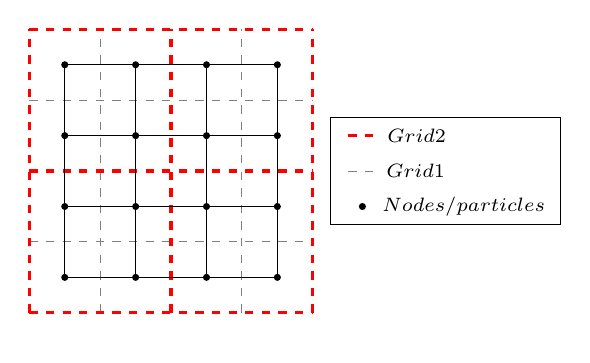
\begin{tikzpicture}[scale=0.9]
  \draw (0,0) --(3,0)--(3,3)--(0,3)--(0,0);
  \draw[white] (0.,0) -- (0,-0.8);
  %%% Grid 1
  \foreach \y in {-0.5,0.5,...,3.5} 
  \draw[dashed,gray] (-0.5,\y) -- (3.5,\y);
  \foreach \x in {-0.5,0.5,...,3.5} 
  \draw[dashed,gray] (\x,-0.5) -- (\x,3.5);
  %%% Grid 2
  \foreach \y in {-0.5,1.5,...,3.5} 
  \draw[dashed,Red,very thick] (-0.5,\y) -- (3.5,\y);
  \foreach \x in {-0.5,1.5,...,3.5} 
  \draw[dashed,Red,very thick] (\x,-0.5) -- (\x,3.5);
  \foreach \y in {0.,1.,...,3.} 
  \foreach \x in {0.,1.,...,3.} 
  \fill (\x,\y) circle(0.05);
  \foreach \y in {0.,1.,...,3.} 
  \draw (0,\y) -- (3.,\y);
  \foreach \x in {0.,1.,...,3.} 
  \draw (\x,0) -- (\x,3);
  \draw (3.75,0.75) rectangle (7.,2.25);
  \fill (4.2,1.) circle (0.05) node [right] {\scriptsize$ \: \: \text{Nodes / particles}$};
  \draw[dashed,gray] (4.,1.5) -- (4.4,1.5) node [right] {\scriptsize$\color{black} \text{Grid 1}$};
  \draw[dashed,very thick,Red] (4.,2.) -- (4.4,2.) node [right] {\scriptsize$\color{black} \text{Grid 2}$};
\end{tikzpicture}


%%% Local Variables:
%%% mode: latex
%%% TeX-master: "../manuscript"
%%% End:
}
  \caption{Geometry, loading and boundary conditions for the tensile impact problem on a two-dimensional elastic medium.}
  \label{fig:2D_planeStrain}
\end{figure}
The MPM and the DGMPM using CTU method are compared to a $Q1$ finite element (bilinear approximation) solution obtained with the code Cast3M Drexus \cite{Castem}.

The domain is discretized such that material points are equivalent to finite element nodes, that is: $l\times l \equiv 28 \times 28$ particles and nodes. Moreover, two arbitrary grids are used for the DGMPM so that either one or four material points lie in every cells according to the situations depicted in figure \ref{fig:2D_planeStrain}\subref{subfig:2d_meshes}.
\begin{figure}[h!]
  \centering
  

\begin{figure}\centering
  \begin{tikzpicture}
    \begin{groupplot}[group style={group size=3 by 2,
        ylabels at=edge left, yticklabels at=edge left,
        horizontal sep=.5ex,
        vertical sep=2ex,},
      enlargelimits=0,
      xmin=0.,xmax=1., ymin=-0.,ymax=1.
      ,axis on top,scale only axis,xtick=\empty,ytick=\empty,width=0.25\linewidth,
      colorbar style={
        title style={
          font=\scriptsize,
          at={(1,.5)},
          anchor=north west
        },yticklabel style={font=\scriptsize}
      ,at={(current axis.south east)},anchor=south west
      }]
      %% FIRST ROW (time 1 = 3.5e-4s)
      %%% RANGE -1.6e7 -- 2.9e8
      \nextgroupplot[ylabel={$t=3.5\times 10^{-4} \:s.$},title={FEM}]\addplot graphics[xmin=0.,xmax=1., ymin=-0.,ymax=1.] {chapter4/pngFigures/fem_stress_78.png};
      \nextgroupplot[title={DGMPM 1ppc}]\addplot graphics[xmin=-0.,xmax=1., ymin=-0.,ymax=1.] {chapter4/pngFigures/dgmpm1ppc_stress_78.png};
      \nextgroupplot[title={DGMPM 4ppc},
      colorbar,colorbar style={
        title= {$\sigma_{11}\: (GPa)$},
        ytick={-1.6e-2,2.9e-1},
        %yticklabels={0,0.5,1},
      }]
      \addplot[scatter,scatter src=y,mark size=0.pt] coordinates {(0.,-1.6e-2) (0.,2.9e-1)};% Fake extreme values to fix scale
      \addplot graphics[xmin=-0.,xmax=1., ymin=-0.,ymax=1.] {chapter4/pngFigures/dgmpm4ppc_stress_78.png};

      %% SECOND ROW (time 2 =1.e-3s)
      %%% RANGE -2.9e7 -- 3.5e8
      \nextgroupplot[ylabel={$t=1.0\times 10^{-3} \:s.$}]\addplot graphics[xmin=0.,xmax=1., ymin=-0.,ymax=1.] {chapter4/pngFigures/fem_stress_231.png};
      \nextgroupplot[]\addplot graphics[xmin=-0.,xmax=1., ymin=-0.,ymax=1.] {chapter4/pngFigures/dgmpm1ppc_stress_231.png};
      \nextgroupplot[colorbar,colorbar style={
        title= {$\sigma_{11}\: (GPa)$},
        ytick={-2.9e-2,3.5e-1},
        %yticklabels={0,0.5,1},
      }]
      \addplot[scatter,scatter src=y,mark size=0.pt] coordinates {(0.,-2.9e-2) (0.,3.5e-1)};% Fake extreme values to fix scale
      \addplot graphics[xmin=-0.,xmax=1., ymin=-0.,ymax=1.] {chapter4/pngFigures/dgmpm4ppc_stress_231.png};
      
    \end{groupplot}
  \end{tikzpicture}
  \caption{time $t=3.5e-4s$}
  \label{fig:2delast_comparison1}
\end{figure}



%%% Local Variables:
%%% mode: latex
%%% TeX-master: "../mainManuscript"
%%% End:

  \caption{Isovalues of longitudinal stress $\sigma_{11}$ solution of the tensile impact problem in a two-dimensional elastic medium. Comparison between FEM (CFL=0.9), DGMPM-CTU using 1ppc (CFL=1) or 4ppc (CFL=0.23), and MPM using 1ppc (CFL=0.7).}
  \label{fig:2delast_comparison}
\end{figure}
Figure \ref{fig:2delast_comparison} shows the isovalues of longitudinal stress $\sigma_{11}$ in the two-dimensional medium at two different times with the traction force set to $\sigma^d=200\: Mpa$. The first and second lines of plots respectively corresponds to the stress profile before and after reflection of the pressure wave on the right boundary of the domain.
Unlike FEM and MPM, DGMPM solutions do not exhibit oscillations. Nevertheless, the decrease in the CFL number involved by 4ppc yields a less accurate resolution of the jump discontinuity carried by the longitudinal pressure wave than for 1ppc.

On the other hand, the propagation of waves in both directions $\vect{e}_1$ and $\vect{e}_2$ leads to a cylindrical profile of the longitudinal stress that is almost indentically described by FEM and DGMPM with 1ppc, even after reflection of the fixed boundary. On the other hand, the smoothness of DGMPM solutions using 4ppc and the oscillations in MPM results prevent distinguishing this structure.

\begin{figure}[h!]
  \begin{tikzpicture}
  \begin{groupplot}[group style={group size=2 by 1,
ylabels at=edge left, yticklabels at=edge left,horizontal sep=1.5ex,
xticklabels at=edge bottom,xlabels at=edge bottom},
ymajorgrids=true,xmajorgrids=true,xlabel=$x \: (m)$,
axis on top,scale only axis,width=0.43\linewidth, every x tick scale label/.style={at={(xticklabel* cs:1.05,0.75cm)},anchor=near yticklabel},ymin=-0.5e6,ymax=.5e9,xmin=0,xmax=3]
\nextgroupplot[ylabel=$\sigma_{11}\: (Pa)$,title={$t=2.5 \times 10^{-4} \: s$},every y tick scale label/.style={at={(-0.,1.1)}}]
\addplot[Red,very thick,no markers] table[x=Points:0,y=S11] {section4/csvFiles/2delast_fem_115.csv};

\addplot[Blue,very thick,mark=+,only marks,mark size=3pt] table[x=Points:0,y=stress_11] {section4/csvFiles/2delast_ctu1ppc_115.csv};
\addplot[Purple,very thick,mark=asterisk,only marks,mark size=2pt] table[x=Points:0,y=stress_11] {section4/csvFiles/2delast_ctu4ppc_115.csv};
\addplot[Orange,very thick,mark=x,only marks,mark size=3pt] table[x=Points:0,y=mpm_S11] {section4/csvFiles/2delast_mpm_115.csv};

\nextgroupplot[legend style={at={($(0.22,-0.3)+(1.cm,0cm)$)},legend columns=2},xlabel=$x (m)$,title={$t=1.0 \times 10^{-3} \: s$},ytick scale label code/.code={}]
\addplot[Red,very thick,no markers] table[x=Points:0,y=S11] {section4/csvFiles/2delast_fem_338.csv};
\addplot[Blue,very thick,mark=+,only marks,mark size=3pt] table[x=Points:0,y=stress_11] {section4/csvFiles/2delast_ctu1ppc_338.csv};
\addplot[Purple,very thick,mark=asterisk,only marks,mark size=2pt] table[x=Points:0,y=stress_11] {section4/csvFiles/2delast_ctu4ppc_338.csv};
\addplot[Orange,very thick,mark=x,only marks,mark size=3pt] table[x=Points:0,y=mpm_S11] {section4/csvFiles/2delast_mpm_338.csv};
\addlegendentry{fem}
\addlegendentry{ctu 1ppc}
\addlegendentry{ctu 4ppc}
\addlegendentry{mpm}
   
  \end{groupplot}
\end{tikzpicture}


%%% Local Variables:
%%% mode: latex
%%% TeX-master: "../../aRenaud"
%%% End:




































%%% Local Variables:
%%% mode: latex
%%% TeX-master: "../../mainManuscript"
%%% End:

  \caption{tes}
  \label{fig:elastlines}
\end{figure}


%%% Local Variables:
%%% mode: latex
%%% TeX-master: "../mainManuscript"
%%% End:
